%%%%%%%%%%%%%%%%%%%%%%%%%%%%%%%%%%%%%%%%%%%%%%%%%%%%%%%%%%%%%%%%%%%%%%%%%%%%
\documentclass[dvipdfmx,a4j]{jarticle}

\usepackage{jsaisig}
\usepackage{amsmath,amssymb}
\usepackage{graphicx}
\usepackage{bm}
\usepackage{booktabs}
\usepackage{multirow}
\usepackage{color}

\setlength{\textfloatsep}{10pt}
\setlength{\abovecaptionskip}{3pt}
\setlength{\belowcaptionskip}{0pt}
\renewcommand{\baselinestretch}{0.95}

\newcommand{\argmax}{\mathop{\rm argmax}\limits}

%%%%%%%%%%%%%%%%%%%%%%%%%%%%%%%%%%%%%%%%%%%%%%%%%%%%%%%%%%%%%%%%%%%%%%%%%%%

\begin{document}

\title{回答履歴を考慮した強化学習に基づく適応型テスト}
\etitle{Adaptive Testing Based on Reinforcement Learning Considering Response History}

\author{柴沼 厳 \ \ 宇都 雅輝}

\affiliation{%
	電気通信大学\\
	The University of Electro-Communications}

\abstract{

項目反応理論（Item Response Theory: IRT）に基づくコンピュータ適応型テスト（Computerized Adaptive Testing: CAT）では，受検者の能力推定の効率性が項目選択手法に強く依存する．一般的な項目選択手法としてはフィッシャー情報量最大化による方法が知られているが，近年，深層強化学習を用いたDeep Q-Network（DQN）に基づく項目選択手法が提案され，能力推定の精度と効率性の改善が報告されている．しかし，従来のDQNに基づく手法では，強化学習の状態変数として現時点での能力推定値のみを用いるため，受検者のこれまでの回答パターンに含まれる情報を十分に活用できていない．そこで本研究では，DQNに基づくCATを再定式化し，受検者の回答履歴を状態として利用する Deep Recurrent Q-Networkに基づく項目選択戦略を提案する．シミュレーション実験の結果，テスト全体わたるRMSEの平均値において提案手法は従来手法を上回る数値を示した．
}

\maketitle
\thispagestyle{empty}

\section{はじめに}\label{sec:intro}

コンピュータ適応型テスト（Computerized Adaptive Testing: CAT）は，出題される項目が受検者の回答行動に応じて適応的に変化するテスト方式であり，コンピュータを用いた試験（Computer-based Testing）において広く利用されている．一般にCATは項目反応理論（Item Response Theory: IRT）の利用を前提に設計されることが多い~\cite{vanderlinden2016}．IRTに基づくCATでは，受検者に項目を出題して反応データが得られるために，IRTに基づいて受検者の能力を推定し，その能力に適した項目が次の項目として選択・出題される．このような適応的な出題機構により，CATは従来の固定項目型のテスト形式と比べて，より少ない項目数で受検者の能力を高精度に推定できる利点を有する~\cite{frey2023,wainer2000}．

他方で，CATにおける能力測定の効率性は，項目選択手法に強く依存するため，その手法開発が重要な研究テーマとなる．最も標準的な項目選択手法としては，フィッシャー情報量を最大化する項目を選択する最大フィッシャー情報量手法（Maximum Fisher Information: MFI）が知られている~\cite{lord1980}．MFIは現在の能力推定値に対する漸近誤差分散の逆数を最大化するという原理に基づくが，暫定の能力推定値が真の能力値から大きく乖離している場合などでは，適切な項目を選択できないといった問題が知られている~\cite{chang1996}．他方で，この問題への対処を目的として，尤度重み付きフィッシャー情報量（Fisher Information Weighted by the Likelihood: FIWL）~\cite{veerkamp1997} や，尤度重み付きKullback-Leibler情報量（Kullback-Leibler information weighted by the Posterior: KLP）~\cite{chang1996} などに基づく項目選択手法も提案されてきた．

しかし，このような従来の項目選択手法には，共通する二つの課題が残る．一つ目の課題としては，全体最適ではなく局所最適な項目選択を行う点が挙げられる．これは，次の1項目の選択行動のみを最適化対象としており，その先の項目選択全体の影響が考慮されないために生じる課題である．二つ目の課題は，項目選択の方略をデータドリブンで柔軟に構築できない点である．対象の項目集合に対する過去の受検者集団の反応データが得られる場合，そのデータを用いて能力推定の効率や精度を最大化する項目選択方略を設計できる可能性があるが，それらがMFIやFIWL，KLPなどに基づく選択手法と一致する保証はない．

これらの課題を解決するアプローチの一つとして，近年，強化学習に基づく項目選択手法が提案されている~\cite{ghosh2021,nurakhmetov2019,shin2022,wang2024}．
これらの手法では，過去の項目反応データから動的に項目選択方略を学習できるとともに，将来の項目選択全体で得られる情報量の期待値を最大化するように項目を選択するため，局所最適に留まらない項目選択が可能となる．
強化学習に基づく最新の項目選択手法の一つとして，Wang et al.~\cite{wang2024} は深層強化学習を用いたDeep Q-Network（DQN）に基づく項目選択手法を提案している．
この手法では，項目選択問題をマルコフ決定過程（Markov Decision Process: MDP）として定式化し，DQNによるQ関数（行動価値関数）の近似を通して，項目選択を実現している．
シミュレーション実験と実データ実験において，この手法はMFIをはじめとする従来手法より高性能を達成している．

しかし，上記のDQNに基づく従来手法では，DQN内で状態変数として扱われる情報が，IRTに基づく1次元の能力推定値のみとなっており，当該受検者のそれまでの項目反応履歴が利用できない．これは，過去の項目反応履歴が1次元の能力推定値に集約的に表現可能な場合（言い換えると，能力推定に利用しているIRTモデルが項目反応行動を完全に説明可能な場合）には妥当であるが，そうでない場合には．能力推定値に集約できない項目反応情報を取りこぼしてしまい，そのことが学習される項目選択方略の性能に影響を与える可能性がある．そこで本研究では，この課題を解決するために，CATを受験者の項目反応履歴を状態とした MDP として再定式し，Deep Recurrent Q-Network（DRQN）によるQ関数近似に基づいて項目反応履歴を考慮した項目選択を実現する手法を提案する．

\section{項目反応理論に基づくコンピュータ適応型テスト}

本節では，IRTに基づくCATの一般的な方法論について概説する．

\subsection{IRTモデル}

本研究では，CATにおいて能力推定や項目選択に使用されるIRTモデルとして，代表的な二値反応モデルの一つである3パラメータロジスティックモデル（3PLM）の利用を想定する．3PLMでは項目 $i$ に対する受検者の正答確率を次式で定義する．
\begin{equation}
P_i(\theta) = c_i + \frac{1 - c_i}{1 + \exp[-a_i(\theta - b_i)]}
\end{equation}
ここで，$\theta$ は受検者の能力，$a_i$ は識別力パラメータ，$b_i$ は困難度パラメータ，$c_i$ は推測パラメータを表す．以降では，$a_i$，$b_i$，$c_i$を合わせて項目特性値と呼ぶ．

CATでは，項目特性値が予め推定された項目集合（項目バンクと呼ぶ）を用意しておき，そこから受検者にあった項目を適応的に出題する．
具体的には，受検者に項目を出題して回答が得られるたびに，IRTに基づいて受検者の能力を推定し，その能力に適した項目を次の項目として選択・出題する．
なお，項目バンク中の項目特性値の推定は，事前テストなどを通して得られた項目反応データから，周辺最尤推定法などで行われることが一般的である．
また，CATの過程での能力の逐次推定には，最尤法やベイズ推定法が採用されることが一般的である．

%特性値の推定には最尤推定法（MLE）を用い，推定範囲を $[-4, 4]$ とする．テスト開始時の初期特性値は $[-0.5, 0.5]$ の一様分布から無作為に生成する．全回答が正答または全回答が誤答の場合は，Dodd の方法~\cite{dodd1990} に従い，$\hat{\theta}_{l+1} = \hat{\theta}_l + (b_{\max} - \hat{\theta}_l) / 2$（全正答時）または $\hat{\theta}_{l+1} = \hat{\theta}_l + (b_{\min} - \hat{\theta}_l) / 2$（全誤答時）として特性値を更新する．

\subsection{フィッシャー情報量最大化に基づく項目選択手法}

項目選択はCATによる能力推定の効率性や精度に強く影響する中核的な機構として位置付けられる．
代表的な手法であるMFIでは，フィッシャー情報量を最大化するように項目を選択する．
ここで，3PLMを前提とすると，項目 $i$ に対するフィッシャー情報量は次式で定義される．
\begin{equation}
I_i(\theta) =
\frac{a_i^2 (1 - c_i)}
{[c_i + \exp(a_i(\theta - b_i))][1 + \exp(-a_i(\theta - b_i))]^2}
\end{equation}

したがって，$l-1$項目出題した時点での受検者の能力推定値を$\hat{\theta}_l$，その時点での未出題の項目集合を$B_l$とすると，MFIに基づく$l$項目目の項目選択方略は次式で定義される．
\begin{equation}
i_l = \argmax_{i \in B_l} I_i(\hat{\theta}_l)
\end{equation}

しかし，MFIではテスト初期などの暫定の能力推定値が真の能力値から大きく乖離している場合には適切な項目を選択できない可能性がある．この問題への対処としてFIWLの積分値を最大化するような項目を選択する項目選択手法も提案されている~\cite{veerkamp1997}．

しかし，\ref{sec:intro}章で述べた通り，このような従来の項目選択手法の課題として，1）局所最適な選択に陥る点と，2）項目選択の方略をデータドリブンで柔軟に構築できない点が残る．他方で，これらの課題を解決するアプローチとして，強化学習に基づく項目選択手法が提案されている~\cite{ghosh2021,nurakhmetov2019,shin2022,wang2024}．次節では，最新の手法の一つであり，本研究のベースラインとするWang et al.~\cite{wang2024}の手法を紹介する．


%\begin{figure}[t]
%\centering
%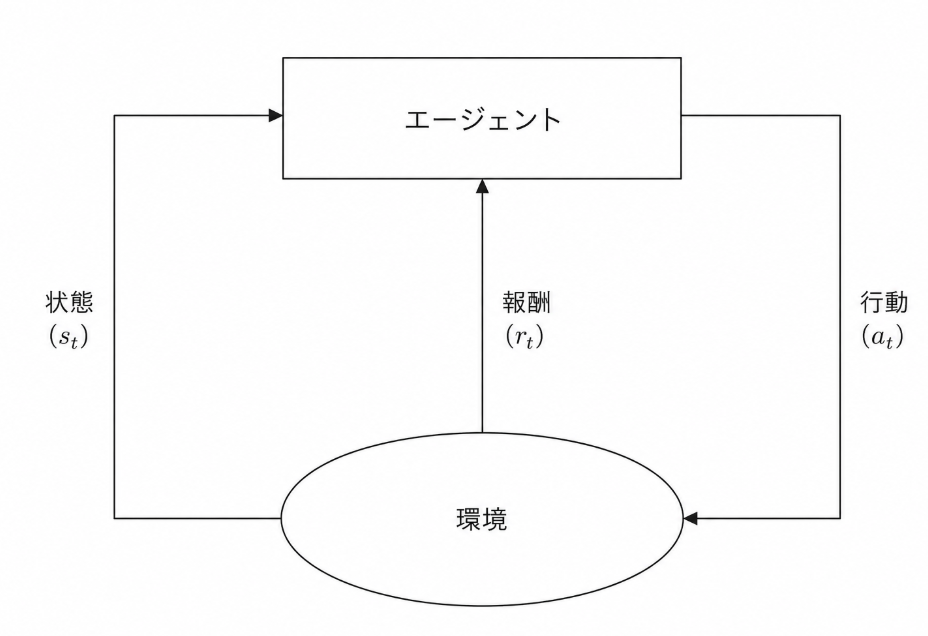
\includegraphics[width=.92\columnwidth]{img/RL.png}
%\caption{強化学習におけるエージェントと環境の相互作用}
%\label{fig:RL}
%\end{figure}


\subsection{強化学習に基づく項目選択手法}

強化学習とはエージェントが環境と相互作用しながら，将来にわたる報酬の重み付き和を最大化するような方策を学習する枠組みである．方策とは，現在の状態に基づいてどのような行動を行うかを確率的に定めるものであり，エージェントとは現在の状態と方策に基づき行動を選択するものである．環境とはエージェントの行動・状態に基づき報酬と次状態を決定するものである．

強化学習において，環境は数理モデルによって記述される．そこでWang ら~\cite{wang2024} は，CAT の項目選択問題を MDP として定式化した．MDP は逐次意思決定問題の数学的枠組みとして広く用いられる，次の状態は現在の状態と行動によってのみ決まるというマルコフ性を仮定したモデルである．Wang ら~\cite{wang2024} は，MDP を用いて項目選択問題を次のように定式化した．

\begin{itemize}
\item 状態：現在の能力推定値 $\hat{\theta}_l$
\item 行動：次に出題する項目（$i_l \in B_l$）の選択行動
\item 報酬：項目 $i_l$ のフィッシャー情報量 $I_{i_l}(\theta)$
\item 環境：IRTに基づく受検者の回答生成と能力推定
\end{itemize}

%\begin{figure}[t]
%\centering
%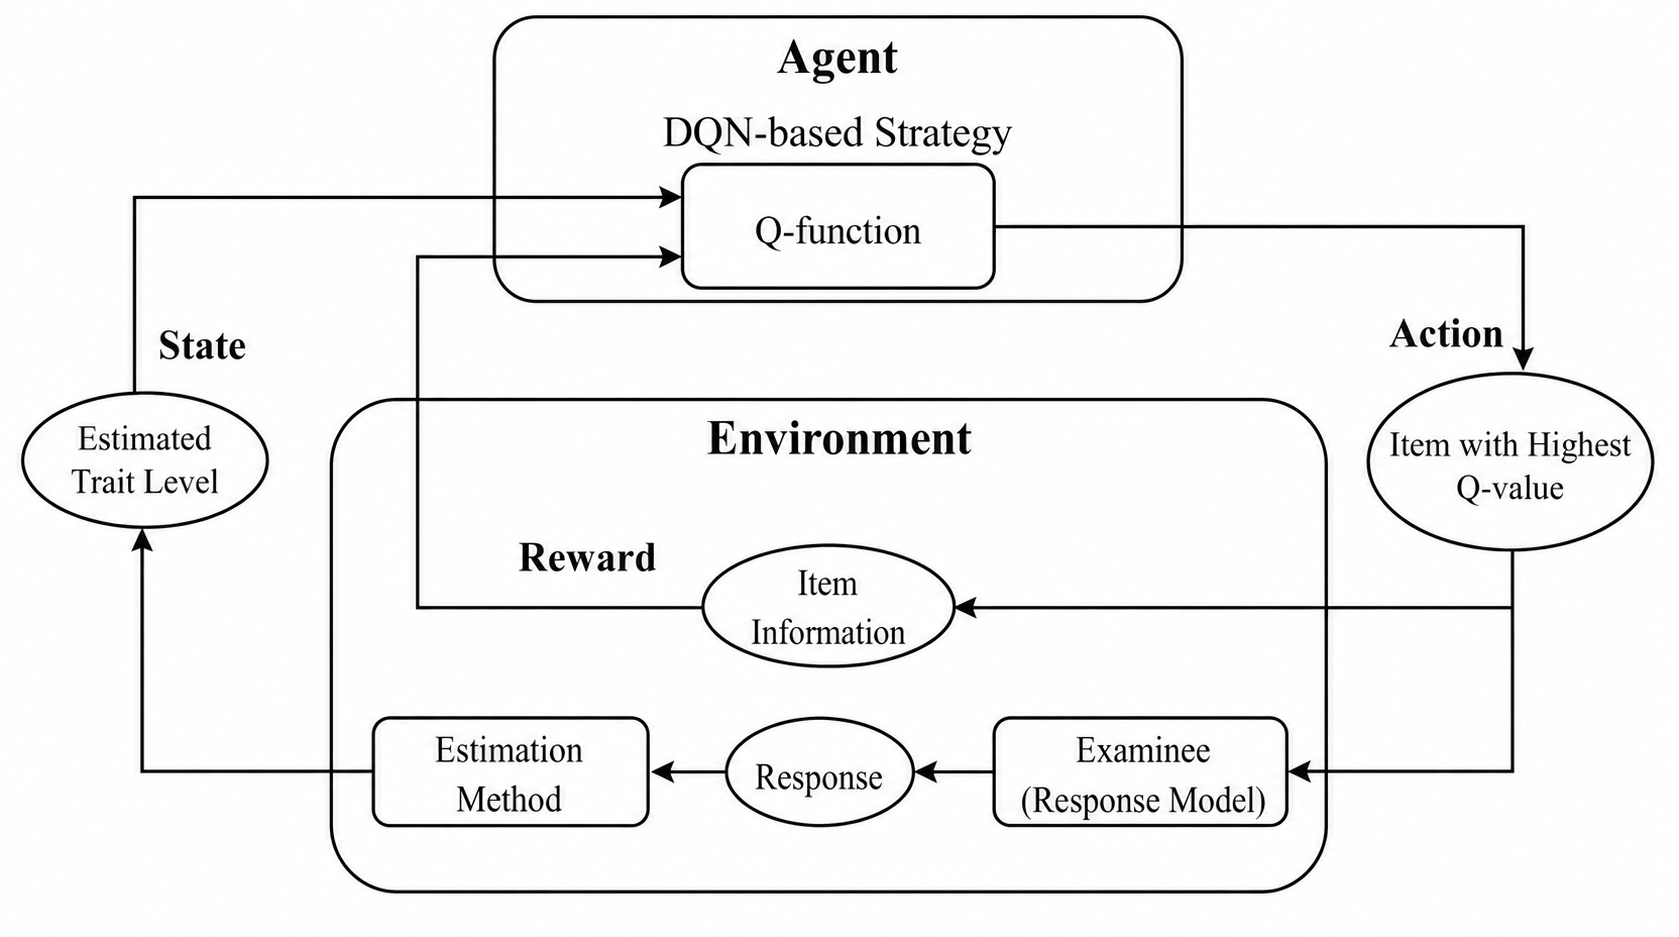
\includegraphics[width=.94\columnwidth]{img/mdp_flow.png}
%\caption{MDPベースの項目選択手法のフローチャート}
%\label{fig:mdp_flow}
%\end{figure}

強化学習で広く使われるアルゴリズムの一つであるQ学習は方策を直接学習するのではなく，Q関数と呼ばれる特定の状態においてある行動を取ったときに得られる期待報酬の総和を表す関数を学習することで最適な方策を導出するアルゴリズムである．

Q 関数は式~\eqref{eq:q_function}で定義される．
\begin{equation}
Q^\pi(\hat{\theta}_l, i_l)
= \mathbb{E}_\pi \left[
I_{i_l}(\hat{\theta}_l)
+ \sum_{k=l+1}^{L} \gamma^{k-l} I_{i_k}(\hat{\theta}_k)
\mid \hat{\theta}_l, i_l
\right]
\label{eq:q_function}
\end{equation}
ここで $\gamma$ は割引率，$L$ はテスト長である．またWang ら~\cite{wang2024} は，このQ関数をニューラルネットワークで近似するDeep Q-Network（DQN）~\cite{mnih2015} を用いて，項目選択方略を学習する手法を提案した．DQN とは，モデルへの入力を状態とし，式~\eqref{eq:td_loss}の損失関数を最小化することでQ関数を近似するアルゴリズムである．

\begin{align}
\mathcal{L}
= \Bigl[
r_l + \gamma \max_{i \in B_{l+1}} Q_{\mathrm{target}}(s_{l+1}, i; \bm{\theta}') \notag\\
- Q_{\mathrm{action}}(s_l, i_l; \bm{\theta})
\Bigr]^2
\label{eq:td_loss}
\end{align}

{\color{red}
[前の説明とここからの説明にギャップがある．Q関数の導入が唐突すぎる．またQ関数を定義して終わりでは意味不明なので，もよくわからないので，全体像との対応関係がより明確になるようにQ関数の役割と説明を書き直すこと．つまり．どのようにこのQ関数を含めた全体の最適化がなされるのかの説明が必要であるということです．3.3ほど具体的でなくていいが，使用されるアルゴリズムとのその概要的な考え方だけ簡潔に述べること．]
}

そして方策には確率 $1-\varepsilon$ で最大のQ値を持つ項目を選択し，確率 $\varepsilon$ でランダムに項目を選択する $\varepsilon$-greedy 法が用いられた．

他方で，このDQNに基づく手法は，状態がIRTに基づく1次元の能力推定値のみとなっており，当該受検者のそれまでの項目反応履歴は利用できないという課題を有する．これは，過去の項目反応履歴が1次元の能力推定値に集約できる，すなわち，能力推定に利用しているIRTモデルが項目反応行動を完全に説明可能な場合には妥当であるが，そうでない場合には，有益な情報を取りこぼす可能性があり，そのことは学習される項目選択方略の性能に影響を与えうる．

\section{提案手法}

本研究では，上記の課題を解決するために，各受検者の項目反応履歴に基づいて項目選択を実現する強化学習ベースの項目選択手法を提案する．具体的には，MDPにおける状態を受験者の項目反応履歴として再定式し，Q関数の近似にDRQNを用いることで，受検者の回答履歴を考慮した項目選択を実現する．

\subsection{DRQN による Q 関数の近似}

Wang ら~\cite{wang2024} と同様に，本研究においてもニューラルネットワークを用いてQ関数を近似することを考える．しかし，Wang ら~\cite{wang2024} らの定式化では状態が能力推定値という非系列的な情報であったのに対し，本研究では状態を受験者の項目反応履歴という系列的な情報として再定式した．そこで本研究では，項目反応履歴を状態として再定式した MDPを解くために，Hausknecht と Stone~\cite{hausknecht2015} が提案した DRQN を用いる．DRQN は DQN の最初の全結合層を LSTM に置き換えたアーキテクチャであり，これまでの受験者の回答系列に基づいて各項目の Q関数の推定を行うことができる．

本研究における DRQN のアーキテクチャは以下の構成である．

\begin{enumerate}
\item Embedding 層：回答を3カテゴリ（0: 誤答，1: 正答，2: 開始トークン）の埋め込み表現に変換する．
\item LSTM 層：埋め込み系列を逐次処理し，隠れ状態を更新する．
\item 全結合出力層：LSTM の出力からアイテムバンク内の全項目に対する Q 値を出力する．
\end{enumerate}

\begin{figure*}[t]
\centering
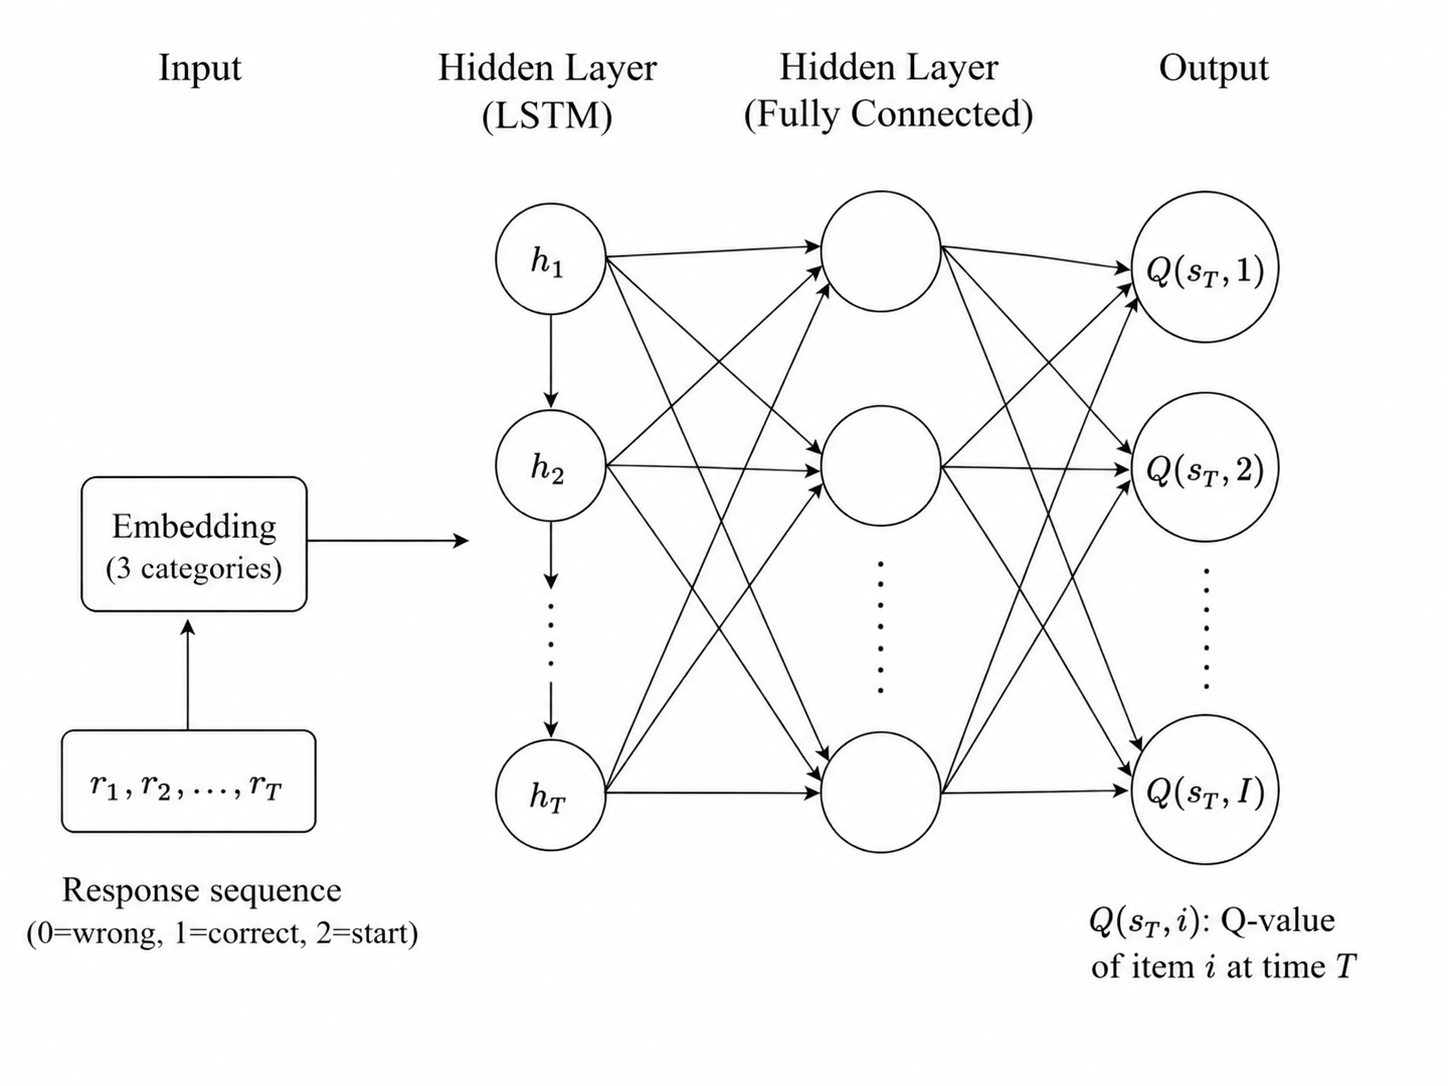
\includegraphics[width=.6\textwidth]{img/drqn_arch.png}
\caption{DRQN のアーキテクチャ．}
\label{fig:drqn_arch}
\end{figure*}

本研究にて使用する DRQN のアーキテクチャを図\ref{fig:drqn_arch}に示す．図\ref{fig:drqn_arch} から分かるように，DRQNにおいて埋め込み表現に変換された項目反応履歴は LSTM で逐次処理される．これにより，受験者の項目履歴をLSTMが内部状態として保持することで これまでの回答履歴に基づいた Q関数の推定を行うことができる．

%\begin{table}[t]
%\centering
%\caption{DQN と DRQN の比較}
%\label{tab:dqn_drqn}
%\scriptsize
%\setlength{\tabcolsep}{3pt}
%\begin{tabular}{p{0.18\columnwidth}p{0.30\columnwidth}p{0.34\columnwidth}}
%\toprule
% & DQN & DRQN \\
%\midrule
%定式化 & MDP & POMDP \\
%状態表現 & 推定特性値 $\hat{\theta}_l$ & 回答履歴 $(o_1,\ldots,o_{l-1})$ \\
%ネットワーク & 全結合ネットワーク & Embedding + LSTM + 全結合 \\
%入力次元 & 1 & 可変長系列 \\
%\bottomrule
%\end{tabular}
%\end{table}

次節にて，DRQN の学習アルゴリズムについて説明する．

\subsection{学習アルゴリズム}

先行研究~\cite{hausknecht2015} に倣いDRQNの学習には，安定化を目的に 経験再生(Experience Replay) という手法を用いる．経験再生とは，DRQNで近似された Q関数の値と $\varepsilon$-greedy 法によって生成された項目反応履歴，選択された項目，報酬の系列の3つの情報をリプレイメモリに蓄積した後，ランダムサンプリングして損失関数を最小化することでネットワークのパラメータを更新する手法である．DRQN はエピソード単位，すなわち1人の受検者のテスト全体を1エピソードとて ネットワークのパラメータを更新する．ただし，推論時には項目反応履歴を1ステップずつDRQNに入力し，各ステップでのQ値を計算することで次の項目選択を行う．また，方策には Wang ら~\cite{wang2024} と同様に$\varepsilon$-greedy 法を用いる.

学習の手順は以下の様にまとめることができる．

\begin{enumerate}
\item 学習用の真の特性値 $\theta_n \sim N(0,1)$

（$n = 1,\ldots,N_{\mathrm{training}}$）を事前に一括生成する．

\item 受検者 $n = 1, \ldots, N_{\mathrm{training}}$ について順に，以下のシミュレーションを行いエピソードを生成する．
  \begin{enumerate}
    \item 各決定ステップ $l = 1, \ldots, L$ において，DRQNによって近似されたQ関数の値と $\varepsilon$-greedy 法を用いて未出題項目から項目 $i_l$ を選択する．
    \item 3PLM に基づき，真の特性値 $\theta_n$ を用いて回答 $o_l \in \{0,1\}$ を確率的に生成する．
    \item 報酬 $r_l = I_{i_l}(\theta_n)$ を，真の特性値 $\theta_n$ におけるフィッシャー情報量として計算する．
  \end{enumerate}
  1エピソード分の回答系列・行動系列・報酬系列をリプレイメモリに保存する．

\item リプレイメモリに $m$ 件以上のエピソードが蓄積されたら，$m$ 件のミニバッチをサンプリングし，式~\eqref{eq:td_loss}の損失関数で Q-Network のパラメータを更新する．
$\tau$ 回の更新ごとにターゲットネットワークのパラメータを同期する．

\item 手順2〜3を $N_{\mathrm{training}}$ 回繰り返す間，一定間隔でバリデーションを行い，最良モデルを保存する．
\end{enumerate}


\section{シミュレーション実験}

\subsection{実験設定}

\paragraph{アイテムバンクの生成}

Wang ら~\cite{wang2024} のシミュレーション設定に基づき，各アイテムバンクを200項目で生成した．項目パラメータの分布は以下の通りである．
\begin{itemize}
\item 識別力：$a \sim N(1.2, 0.25)$（$a > 0$）
\item 困難度：$b \sim N(0, 1)$
\item 疑似推測：$c \sim N(0.25, 0.02)$（$0 < c < 1$）
\end{itemize}

項目のパラメータ $a$ と $b$ は通常相関していることを考慮しパラメータ間に相関のないアイテムバンク（無相関アイテムバンク，$r_{ab}=0$）と 相関のあるアイテムバンク（相関アイテムバンク，$r_{ab}=0.5$）の2種類を各3バンク，計6バンク生成した．各バンクに対して，5000名の受検者の真の特性値を標準正規分布 $N(0,1)$ から生成し各手法の性能評価に用いた．

\paragraph{比較手法}


本研究ではMFI~\cite{lord1980}，DQN~\cite{wang2024}，DRQN(提案手法)~\cite{hausknecht2015} の3手法を比較する．ただし，DQNは学習用の真の特性値を一様分布から生成したもの（DQN\_uniform）と正規分布から生成したもの（DQN\_normal）の2種類を用意し，DRQNの学習には一様分布のみを使用した．

%\paragraph{強化学習手法のハイパーパラメータ}
%
%DQN と DRQN の学習設定を表~\ref{tab:hyperparams} に示す．
%
%\begin{table}[t]
%\centering
%\caption{DQN と DRQN のハイパーパラメータ}
%\label{tab:hyperparams}
%\scriptsize
%\setlength{\tabcolsep}{3pt}
%\begin{tabular}{p{0.28\columnwidth}p{0.22\columnwidth}p{0.33\columnwidth}}
%\toprule
%パラメータ & DQN & DRQN \\
%\midrule
%ネットワーク構造 & \shortstack[l]{1$\to$50\\$\to$30$\to$200} & \shortstack[l]{Embedding(3,16)\\$\to$LSTM(64)\\$\to$Linear(200)} \\
%学習データ数 $N_{\mathrm{training}}$ & 1,000 & 1,000 \\
%テスト長 $L$ & 40 & 40 \\
%割引率 $\gamma$ & 0.1 & 0.1 \\
%リプレイメモリサイズ $N_D$ & 1,000 & 1,000 \\
%ミニバッチサイズ $m$ & 128 & 128 \\
%ターゲット更新間隔 $\tau$ & 40 & 40 \\
%学習率 & 0.001 & 0.001 \\
%$\varepsilon$ & 0.1 & 0.1 \\
%バリデーション間隔 & 50 & 50 \\
%バリデーション数 & 200 & 200 \\
%学習データ分布 & $N(0,1)$ & $N(0,1)$ \\
%報酬 & $I_{i_l}(\theta)$ & $I_{i_l}(\theta)$ \\
%\bottomrule
%\end{tabular}
%\end{table}

%DQN では全てのネットワークパラメータに正値制約を適用し，Q 値が正であることを保証する．DRQN では出力層の重みとバイアスのみに正値制約を適用し，さらに勾配クリッピング（最大ノルム 1.0）を導入して学習を安定化させる．

\paragraph{評価指標}

シミュレーション実験にて以下の2つの指標を用いて，各手法の推定精度を評価する．

\begin{equation}
\mathrm{Bias} = \frac{1}{N} \sum_{n=1}^{N} (\hat{\theta}_n - \theta_n)
\end{equation}
\begin{equation}
\mathrm{RMSE} = \sqrt{\frac{1}{N} \sum_{n=1}^{N} (\hat{\theta}_n - \theta_n)^2}
\end{equation}

%\begin{equation}
%\mathrm{MAE} = \frac{1}{N} \sum_{n=1}^{N} \lvert \hat{\theta}_n - \theta_n \rvert
%\end{equation}

\subsection{結果}

無相関アイテムバンク（$r_{ab}=0$）と相関アイテムバンク（$r_{ab}=0.5$）の各ステップにおけるRMSE，Biasの平均値を図\ref{fig:results_rmse}\ref{fig:results_bias}に示す．

\begin{figure*}[t]
\centering
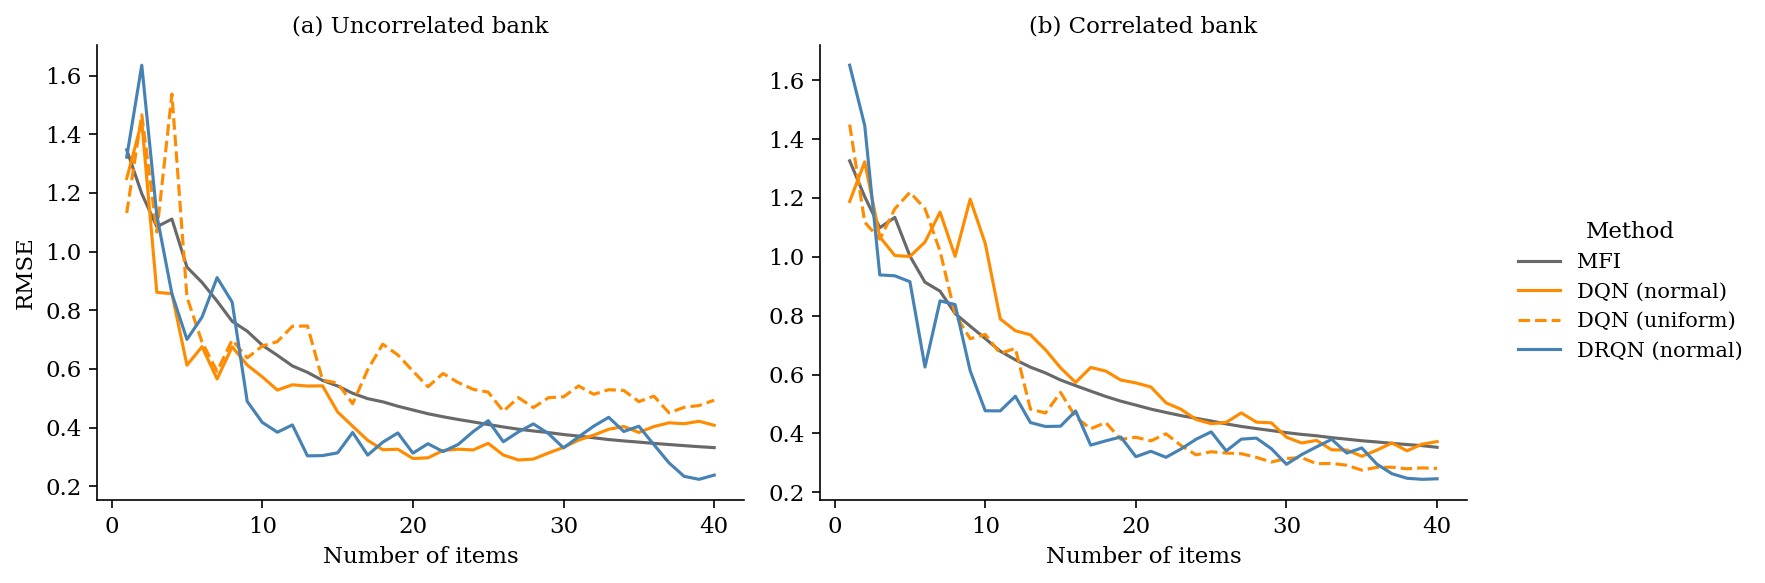
\includegraphics[width=\textwidth]{img/plot_results_rmse.png}
\caption{各ステップにおける RMSE の推移（無相関バンク・有相関バンク，バンク1〜3平均）}
\label{fig:results_rmse}
\end{figure*}

\begin{figure*}[t]
\centering
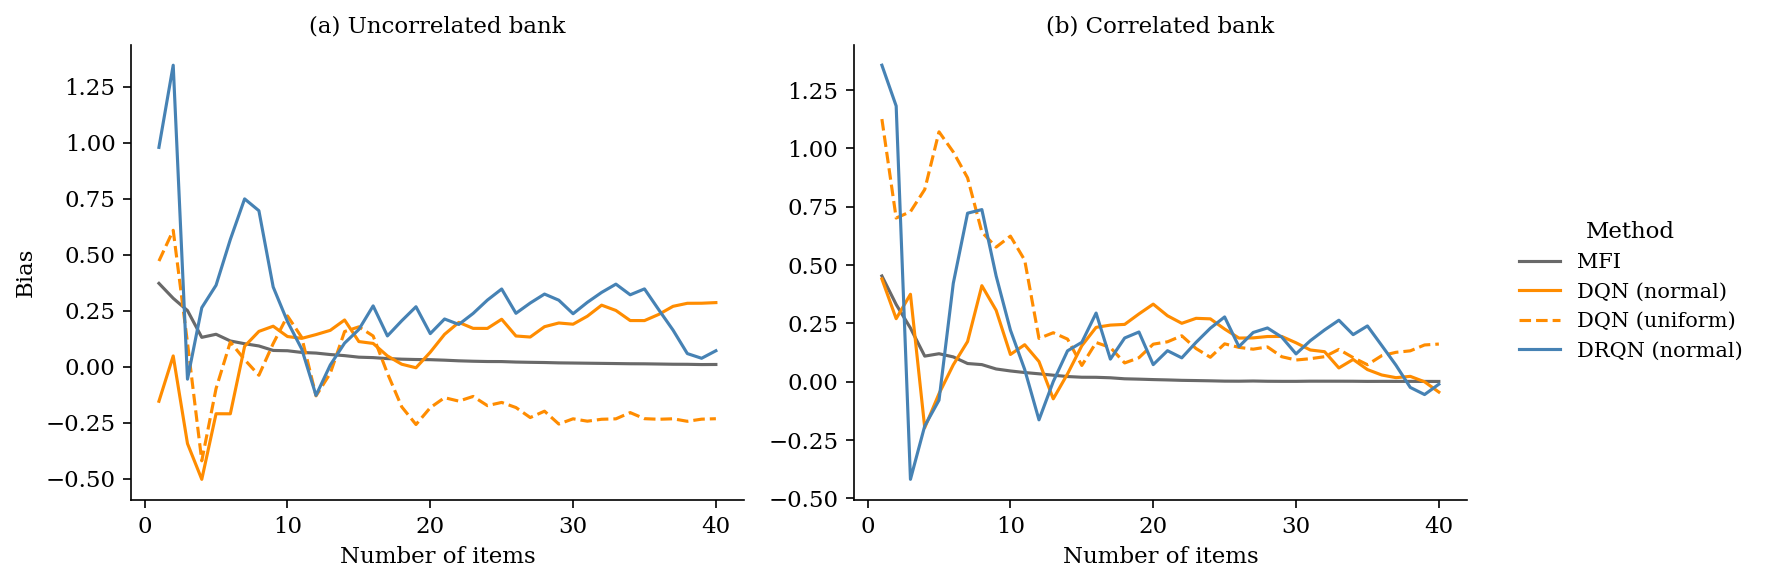
\includegraphics[width=\textwidth]{img/plot_results_bias.png}
\caption{各ステップにおける Bias の推移（無相関バンク・有相関バンク，バンク1〜3平均）}
\label{fig:results_bias}
\end{figure*}

図\ref{fig:results_bias}から分かるように，テスト初期の10 ～ 15問目において提案手法は無相関アイテムバンクで RMSE が DQN\_normal と比較して最大 43\% 改善(DQN\_uniformと比較して最大60\%改善)し，相関アイテムバンクで RMSEが DQN\_uniform と比較して最大 35\% 改善(DQN\_normalに比べて最大55\%改善)するなど，提案手法はテスト初期において 既存手法の DQN よりも大幅に精度が高いことが確認できる．

また，テスト全体における平均RMSEを見ると無相関アイテムバンクでは 提案手法は DQN\_uniform に比べて 約10\% の改善を示し，DQN\_normal とは同程度の精度を示した．相関アイテムバンクにおいては 提案手法 DQN\_uniform を約14\%上回る精度を示し, DQN\_normal を約5\%上回る精度を示した．


%3. MFIが40問選択時点にて達成したRMSEを 無相関アイテムバンクにて 13問目(DQN\_normalは18問目,DQN\_uniformは到達せず)にて達成し, 相関アイテムバンクにて 20問目(DQN\_normalは33問目,DQN\_uniformは24問目)にて達成するなど, 提案手法はテスト初期において 既存手法の MFI よりも大幅に精度が高いことが確認できる.

%4. 既存手法である DQN の性能は, 使用するアイテムバンクの項目パラメータの相関の有無に大きく依存し, 学習に使用する真の特性値の分布を適切に選択する必要がある. 学習に使用する真の特性値の分布の選び方次第では, MFI よりも大きく性能が劣る可能性があることも図より確認できる. 一方, シミュレーション実験において提案手法の学習に使用した真の特性値の分布は正規分布に固定されているにも関わらず, 安定して MFI よりも高い精度を示していることから, 提案手法は学習に使用する真の特性値の分布に対して比較的ロバストである可能性が示唆される.


\section{おわりに}

本研究は，IRTに基づく CAT の項目選択を Wang ら~\cite{wang2024} の定式化における状態を受験者の回答履歴に置き換える形で再定式し，Q関数をDRQNで近似する手法を提案した．3PLMによって生成されたシミュレーションデータを用いて既存手法と提案手法の比較を行った結果，テスト全体における平均RMSEは提案手法が既存手法のDQNを約5〜14\%上回る精度を示した．特に，テスト初期の10 〜 15問目 において既存手法を大きく上回る性能を示した．本研究での提案手法は，項目パラメータも状態に組み込むことで 項目パラメータを考慮したモデルへ拡張することも可能である．さらに，本研究ではシミュレーション実験において提案手法の性能を評価したが, 今後は実データを用いた実験による性能の検証も必要である．



\bibliographystyle{junsrt}
\bibliography{references}

\end{document}